\documentclass{beamer}
\usetheme{Singapore}
\usepackage[T1]{fontenc}
\usefonttheme{professionalfonts}
\usepackage{amsthm}
\usepackage{times}
\usepackage{graphicx} 

\newtheorem{mydef}{Definition}
\newtheorem{mylemma}{Lemma}
\newtheorem{mytheorem}{Theorem}
\newtheorem{myprep}{Proposition}
\newtheorem{mycor}{Corollary}

%math packages
\usepackage{amsthm}
\usepackage{amsmath}
\usepackage{amssymb}
\usepackage{amsfonts}
\usepackage{mathtools}
\usepackage{tikz}
\usepackage{graphicx}
\usetikzlibrary{shapes.geometric}
\usetikzlibrary{math} 
\usepackage{ifthen}


%%% Algorithmic package
\usepackage{algpseudocode}% http://ctan.org/pkg/algorithmicx
\usepackage{amsmath, color, epsf}
\usepackage[linesnumbered,ruled,vlined]{algorithm2e}
\usepackage{color} 

%Caption packages
\usepackage{caption}
\usepackage{subcaption}
\usepackage{subfiles}
\usepackage{lipsum}
 
%Information to be included in the title page:
\title[Data Engineering assignment]{SpaNPortal}
\author{Siaminou Ioanna}
\date{12/6/2021} 
 
 
\begin{document}
%first slide
\frame{\titlepage}


\begin{frame}
\frametitle{Project Outline}
\tableofcontents
\end{frame}

\section{Introduction}
\begin{frame}
\frametitle{Context}
\begin{enumerate}
\item SpaN is a company that provides an online portal for real estate services.
\item Strategy department of SpaN needs to process the logged property searches acquired by users based on certain criteria.
\item The design of a data lake and and the appropriate pipeline is necessary for better analysis of the data by the Strategy team.
\item The project consists of three distinct parts (Architecture, Implementation, Database Design).
\end{enumerate}
\end{frame}

\section{Architecture}
\begin{frame}
\frametitle{Data \& Dataflows}
\begin{enumerate}
\item The data provided, consisted of a relational database with geographical information, and a series of files, containing user searches logged in a json format.
\item After the preprocessing, appropriate tranformations of the data, extraction of the useful attributes according to the given specifications.
\item The data are enriched with information provided by the second data source, the geography database.
\item Finally, the final dataset is stored in the appropriate format, in order to be stored used efficiently.
\item An overview of my approach follows in the next slide.
\end{enumerate}
\end{frame}

\begin{frame}
\frametitle{Architecture Diagram}
\centering
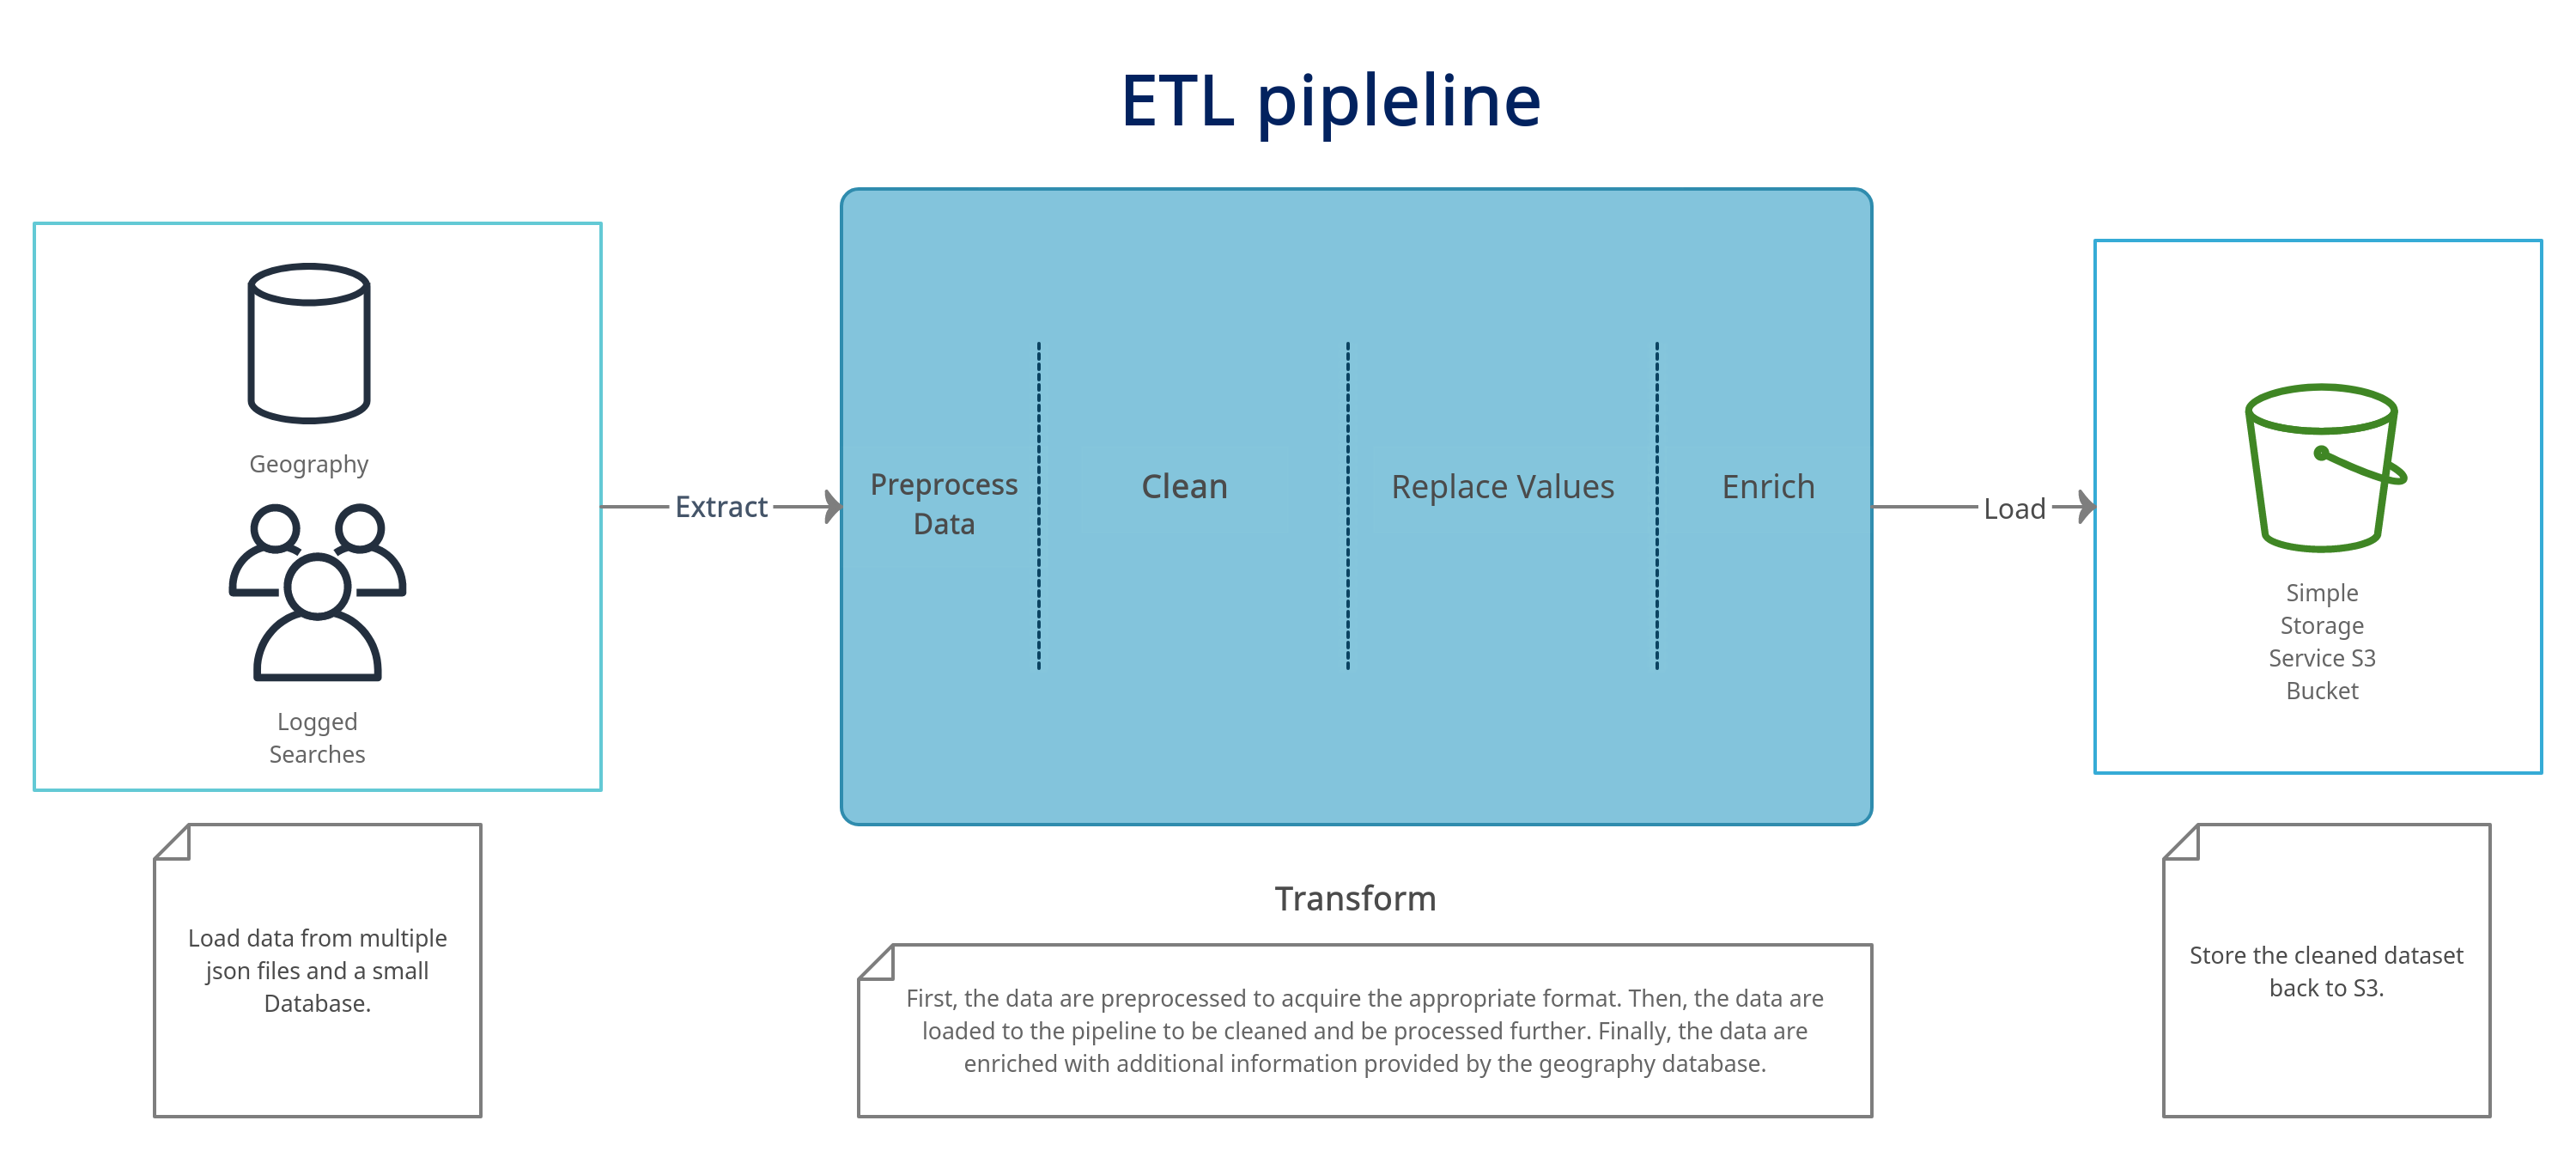
\includegraphics[scale=0.11]{ETL_arch.png}
\end{frame}

\begin{frame}
\frametitle{How data flows through the pipeline?}
\begin{enumerate}
\item After the extraction of the useful data from the data sources, the data are ingested to the transform stage.
\item First, the duplicate records are removed along with the null records.
\item The data are then filtered, to remove any record that correspond to \textit{brokerIDs}.
\item Null values for specific columns are replaced.
\item And finally the data are enriched with additional information.
\end{enumerate}
\end{frame}

\begin{frame}
\frametitle{Data Flow Diagram}
\centering
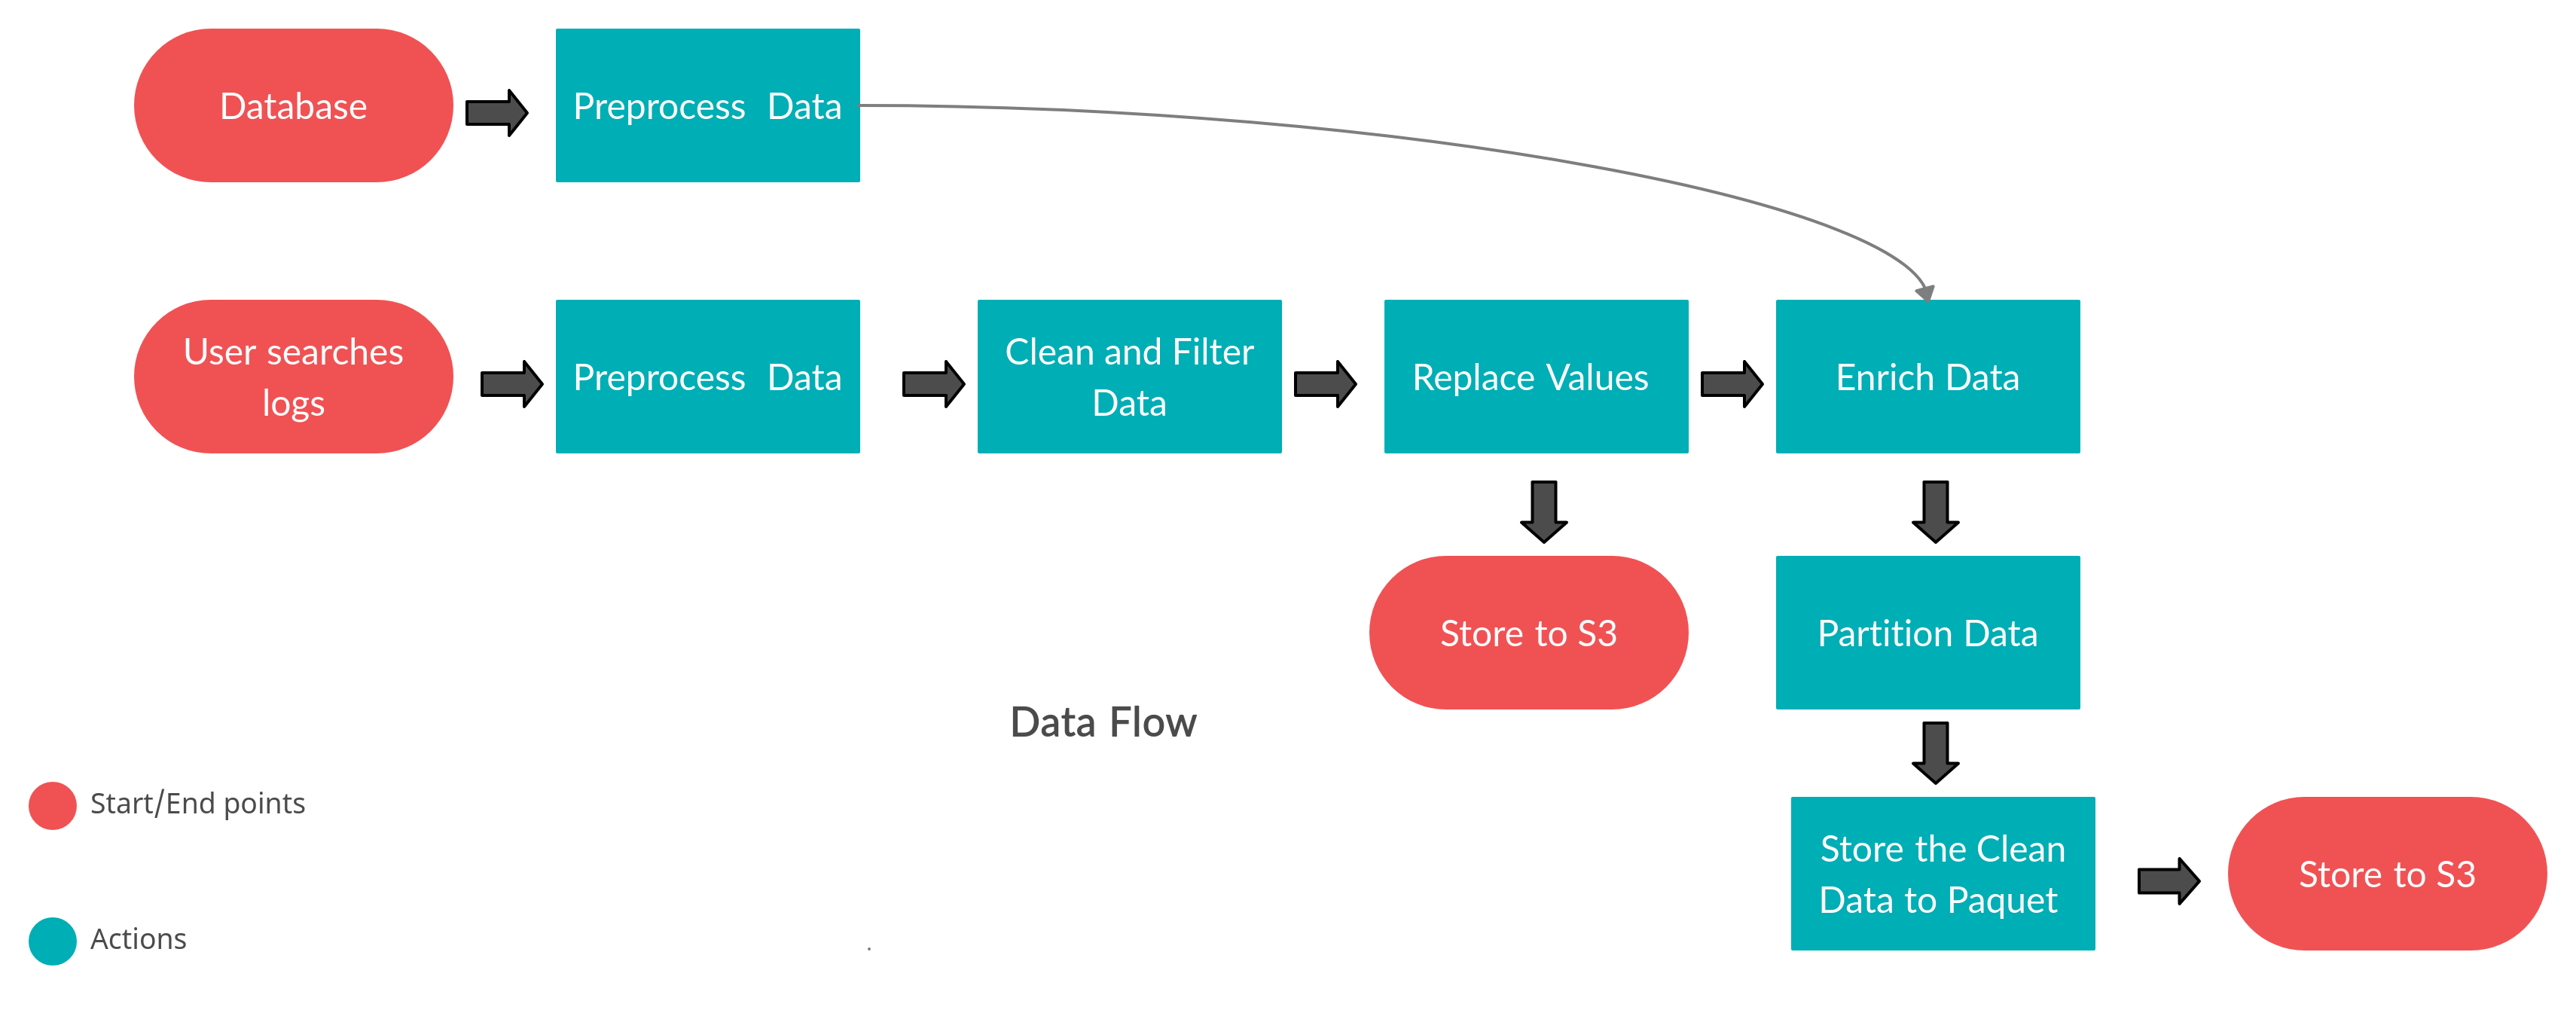
\includegraphics[scale=0.09]{dataFlow.png}
\end{frame}

\section{Implementation}
\begin{frame}
\frametitle{Assignment implementation}
\begin{enumerate}
\item The project is implemented using Python programming language (version: Python 3.8.5).
\item Pyspark is used since it is can perform computation and transformations on data efficiently.
\item The project is accompanied with 2 bash scripts. 
\begin{itemize}
\item To activate a conda environment.
\item To manage the data directories.
\end{itemize}
\item The code is available on my github profile (https://github.com/ninasiam).
\end{enumerate}
\end{frame}

\begin{frame}
\frametitle{Some Notes}
\begin{itemize}
\item The data are preprocessed, in a separate application available in the project directory.
\item Due to a datatype mismatch (false/False) and the interpretation of json objects from pyspark, the json files could not be loaded correctly.
\item I chose to process them separately, using spark RDDs, to keep the pipeline as clean as possible.
\item I am pretty sure that a more efficient way exists (a parameter on pyspark json read function maybe), but at the moment this approach seemed to me straightforward. 
\end{itemize}
\end{frame}

\begin{frame}
\frametitle{More on the implementation}
\begin{itemize}
\item The main script is the etl\_main(), where the sparkSession is initialized.
\item The pipeline functionality (Export, Transform, Load) is implemented on the ETL\_fun.py file.
\item The json file preprocessing is performed by preprocess\_data.py. 
\end{itemize}
\end{frame}

\begin{frame}
\frametitle{Output files}
\begin{itemize}
\item The output datasets (cleaned, enriched) are saved as a parquet files.
\item The Parquet is a column oriented storage file available to any project on the Hadoop ecosystem.
\item Aggregation queries are less time consuming compared to row oriented schemes. 
\end{itemize}
\end{frame}
\end{document}
